\chapter{Implementation}

\tocdata{toc}{$\rightarrow$\textit{Jeremy Sztavinovszki}}
\section{General Architecture}
\addtocontents{toc}{\textit{Jeremy Sztavinovszki}\par}
\textbf{Author: Jeremy Sztavinovszki}
\begin{figure}
	\centering

	\includegraphics[width=\textwidth]{img/RECT-Architecture}
	
	\caption{RECT's Architecture}
	\label{fig:rect-architecture}
\end{figure}

The general Architecture of RECT looks like \ref{fig:rect-architecture}. This is a high level overview of the RECT stack.
In the following sections we will go into more detail about the different parts of the stack and how they were implemented.

\begin{figure}
	\centering

	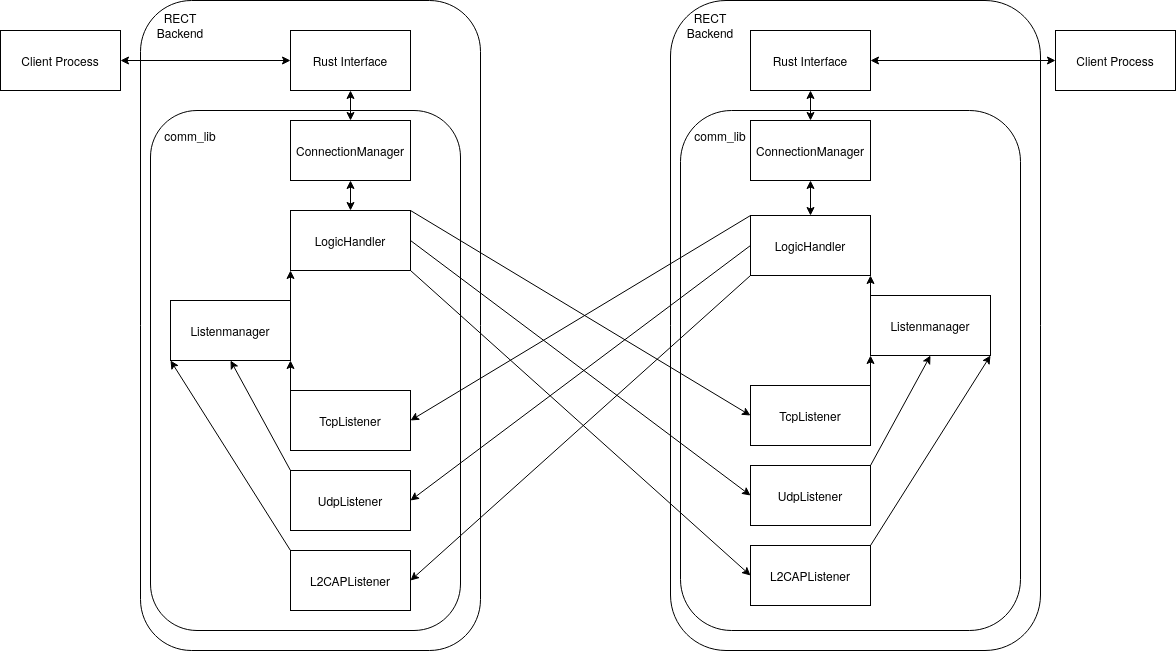
\includegraphics[width=\textwidth]{img/RECT-dataflow}

	\caption{The Flow of Data in RECT}
	\label{fig:rect-dataflow}

\end{figure}

\ref{fig:rect-dataflow} shows how data is sent through the different protocols in RECT.
In this diagram the CommLib takes the part of sending and receiving the data which is to be transmitted to listeners on fixed ports
on other hosts.

\tocdata{toc}{$\rightarrow$\textit{Jeremy Sztavinovszki}}
\section{CommLib}
\addtocontents{toc}{\textit{Jeremy Sztavinovszki}\par}
\textbf{Author: Jeremy Sztavinovszki} 
The Communication Library, or CommLib for short is the part of the RECT stack, that handles all of the communication between the hosts over traditional protocols, like TCP, UDP and BLE.
This requires it to be especially performant. In order to avoid premature optimization however, the first part of this section on the implementation of the CommLib will only cover the first versions
of the code written to get the Library to work. After the first implementation there will be benchmarks and some profiling, in order to get a grasp on which aspects of the library need to be
optimized. The second section will then cover how these results were incorperated into designing a more polished version of the CommLib.

\subsection{Setting up the Library} 
The first steps of setting up the library are more or less the same as in any other rust project. First the project is initialized with \verb+cargo new --lib <rust-name>+. This creates a
new folder with the name specified in \verb+<library-name>+ and generates some files like Cargo.toml and src/main.rs. After this step is done the needed libraries for RECT are added to the
project through \verb+cargo add <dependency-name> -F <dependency-name>/<feature-name>+ these dependencies are the pulled and built by cargo (Rust's build tool) upon the initial build of the
project. The first iteration of the project then had the following dependencies:

\begin{itemize}
	\item tokio
	\item bluer
	\item anyhow
\end{itemize}

All in all the commands used to generate the CommLib project and install all dependencies looked like this:
\newline
\begin{minipage}{\textwidth}
	\begin{lstlisting}[language=bash, caption=Setup Commands for CommLib]
		cargo new --lib CommLib && cd CommLib
		cargo add tokio bluer anyhow enum_dispatch -F tokio/full,bluer/full
		cargo build
	\end{lstlisting}
\end{minipage}

Any application using the CommLib needs to interact with this object in order to be able to use the communication methods provided by the library. 
To achieve this the CommLib provides the following functionality:

\begin{itemize}
	\item Setting a connection to a database, which is used to read the connections configured by the clients.
	\item Receiving simple messages, streams, requests and responses through any of the configured connections.
	\item Sending simple messages, streams, requests and responses through any of the configured connections.
	\item Initiating an update of the connections, which checks changes in the configuration found in the database and the connections, that are currently active in the ConnectionManager.
\end{itemize}

In the following sections the implementation of these functionalities will be covered in more detail.

\subsection{Datatypes for Handling Communication}
% enum_dispatch beschreiben
% verschiedene Typen beschreiben
In order to have a simple and easy to use interface for the CommLib, the library uses a set of different 
types to handle the different kinds of event, which can occur during communication. These types are
as follows:

\begin{itemize}
  \item SimpleMessage
  \item SimpleMessage acknowledgement
  \item Stream subscribe
  \item Stream unsubscribe
  \item Stream data
  \item Request
  \item Request acknowledgement
  \item Response
  \item Response acknowledgement
\end{itemize}

These types are implemented as structs in the CommLib which are part of an enum called Message. This enum uses the enum\_dispatch library
in order to be able to run a set of functions defined in a trait on each of the different structs. Each of the scructs embodies a different
use which will be explained in the following sections.

\subsubsection{SimpleMessage}
The simple message contains a message\_id, which is a 64 bit unsigned integer, a message, which is a vector, or array of bytes,
and a topic which is a String. This message is used to send a message which does not require a response. 
The message\_id is used to identify the message for acknowledgement and to ensure that there are different acknowledgement hashes
for two messages which contain the same data. The topic is used to identify the message on the receiving end.

\subsubsection{SimpleMessage acknowledgement}
The simple message acknowledgement is used to acknowledge the receipt of a simple message. It contains an acknowledgement hash, which is computed
from the message\_id and the data of the message. This hash is then used to verify, that the message was received and insure, that the data in the
message is correct.

\subsubsection{Stream subscribe}
The stream subscribe message is quite minimalistic, only containing a topic, which is a String. This message is used to subscribe to a topic
on the receiving end. Upon receiving this message the recipient will include the sender in the list of subscribers for a given topic. 

\subsubsection{Stream unsubscribe}
Stream unsubscribe is similar to stream subscribe, but is used to unsubscribe from a topic. So insead of adding the sender to the list of subscribers
the recipient will remove the sender from the list of subscribers for a given topic.

\subsubsection{Stream data}
The stream data message is used to send data to a subscriber. This message contains a topic, as well as a message, which is a vector of bytes.

\subsubsection{Request}
The request message is used to send a request to a recipient. It contains a request\_id, which is a 64 bit unsigned integer, a topic, and data, 
which is a vector of bytes. The request\_id is used to identify the request for acknowledgement and to ensure that there are different acknowledgements 
for two requests which contain the same data for the same topic. The topic is used to identify the request on the receiving end and relay it
to the correct recipient process.

\subsubsection{Request acknowledgement}
Similar to the simple message acknowledgement, the request acknowledgement is used to acknowledge the receipt of a request. It contains an acknowledgement
hash, which is computed from the request\_id, topic and the data of the request. This hash is then used to verify, that the request was received and insure, 
that the data in the request is correct. 

\subsubsection{Response}
The response message is used to send a response to a request. It contains a response\_id, which is a 64 bit unsigned integer, a topic, and data,
which is a vector of bytes. The response\_id is used to identify the response for acknowledgment and to relay the response to the correct requesting
process. The topic is used to identify the response on the receiving end.

\subsubsection{Response acknowledgement}
The response acknowledgement is used to acknowledge the receipt of a response. It is the exact same as the request acknowledgement, except for the 
name, which is changed in order to differentiate between the two.


\subsection{Logic for Handling Communication}
% wie werden die verschiedenen Typen verwendet um die Kommunikation zu handlen
% welche software Komponenten gibt es um diese Datentypen zu verwenden 

\subsection{Profiling and Benchmarking}

\subsection{Documentation}
In order to provide an easy understanding of the CommLib and its functionalities, a documentation was created.
Documentation in Rust works by using comments in the code, which are then parsed by the \verb+cargo doc+ command. 
This command generates a folder called \verb+target/doc+ in the project, which contains the documentation in HTML format.
Comments which go into the documentation are written in a specific way.
The following is an example of this: 

\begin{minipage}{\textwidth}
  \begin{lstlisting}[language=Rust, caption=Example of a Documentation Comment]
    //! This is a module/crate-level documentation comment.

    /// This function does something
    /// # Arguments
    /// * `x` - The first parameter
    /// * `y` - The second parameter
    /// # Returns
    /// The sum of `x` and `y`
    fn add(x: i32, y: i32) -> i32 {
      x + y
    }
  \end{lstlisting}
\end{minipage}

As shown in the example, there are crate-, or module-level and general documentation comments. 
The crate-level comments are used to describe a whole crate, or module and provide an overview of the functionality of the crate or module.
The general comments are used to describe functions, structs, enums, traits, etc. and provide 
an explanation of the functionality of the specific item. The documentation for the CommLib can be found in % keine ahnung. appendix a

\tocdata{toc}{$\rightarrow$\textit{Christoph Fellner}}
\section{RECT Database}
\textbf{Author: Christoph Fellner}

\subsection{Why SQLite?}
The choice of a database system is a critical decision in the development of any application, and for RECT, the decision to use SQLite as the backend database 
is grounded in a thoughtful consideration of specific requirements tailored to the nature of small controllers.\newline

Given the diverse landscape of database systems, each with its unique set of advantages and drawbacks, a comprehensive evaluation of options is imperative. 
RECT's emphasis on catering to small controllers immediately guides the criteria for selecting a suitable database. Two key considerations emerge prominently: 
memory efficiency and self-containment.\newline

Small controllers typically operate within constrained resources, making memory efficiency a paramount concern. SQLite, renowned for its lightweight nature and 
minimal memory footprint, aligns seamlessly with this requirement. Its design prioritizes efficiency, ensuring optimal performance even in resource-limited 
environments.\newline

The self-contained nature of SQLite further contributes to its suitability for RECT's use case. Unlike some database systems that necessitate complex setup 
procedures and external dependencies, SQLite operates as a standalone, serverless database engine. This simplicity not only facilitates ease of use but also 
aligns with the desire to avoid intricate configurations. RECT benefits from a database solution that is straightforward to use and configure, enabling a 
seamless integration into the development workflow.\newline

While the focus on memory efficiency and self-containment narrows down the pool of potential databases, SQLite emerges as an optimal choice that strikes a 
balance between these requirements. The careful consideration of these factors positions SQLite as a reliable and pragmatic choice for RECT, providing the 
necessary functionality without introducing unnecessary complexity.\newline

In conclusion, the selection of SQLite for RECT's backend database is a result of a meticulous comparison of different options, with a keen focus on the 
specific needs of small controllers. The prioritization of memory efficiency, self-containment, and ease of use collectively affirm SQLite as the ideal database 
solution, ensuring optimal performance and simplicity in the context of RECT's development environment.

\subsubsection{SQLite}
SQLite\footcite{sqlite} stands out prominently as a frontrunner when it comes to selecting a memory-efficient database, and for good reasons. As a small, fast, 
and serverless database engine, SQLite aligns perfectly with the requirements of applications like RECT, particularly those designed for small controllers.\newline

The serverless nature of SQLite is a noteworthy feature. Unlike some database systems that necessitate a separate server process for operation, SQLite operates 
in a self-contained manner. This characteristic not only simplifies deployment and configuration but also contributes to its efficiency and suitability for 
resource-constrained environments.\newline

Originally developed in the year 2000 by D. Richard Hipp for the US Army, SQLite has evolved into an open-source database engine. Its implementation in the C 
programming language renders it highly portable, allowing it to run seamlessly on a myriad of platforms. This broad compatibility makes SQLite an excellent 
choice for applications that need to be deployed across diverse environments.\newline

The compatibility between SQLite and Rust is facilitated through the rusqlite library, providing a native and ergonomic interface for Rust developers to 
interact with SQLite databases. This seamless integration ensures that the benefits of SQLite, such as its speed and efficiency, can be harnessed effortlessly 
within Rust projects.\newline

Moreover, SQLite offers the flexibility to store the database in memory, enabling rapid access and retrieval of data. The asynchronous access to SQLite 
databases further enhances its versatility, allowing applications like RECT to efficiently manage and interact with data in an asynchronous programming paradigm.\newline

In essence, SQLite's combination of speed, efficiency, serverless operation, and broad platform compatibility positions it as an ideal choice for applications 
that prioritize memory efficiency. For RECT, SQLite, with its inherent qualities and compatibility with Rust through rusqlite, emerges as a robust and fitting 
solution for the backend database, contributing to the overall efficiency and performance of the application.

\subsubsection{PostgreSQL}
Postgres\footcite{postgres}, also known as PostgreSQL, stands as a widely adopted backend database for web applications and websites. Renowned for its robust 
features and scalability, PostgreSQL operates on a client/server architecture, where the database is managed by a dedicated server process. This architecture 
allows multiple clients to interact with the database concurrently, even when accessing the same data simultaneously. The inherent support for handling multiple 
clients makes PostgreSQL particularly well-suited for scenarios where asynchronous access to the database from multiple threads is crucial.\newline

The origins of PostgreSQL trace back to the Berkeley Computer Science Department at the University of California in 1986. Initially named Postgres, the project 
evolved over time and eventually became known as PostgreSQL, although the colloquial shortening to Postgres is still common. In 1996, the project transitioned 
to an open-source model, relying on the contributions of a dedicated group of volunteers for maintenance and improvement. Operating seamlessly on major 
operating systems, PostgreSQL has garnered a reputation for its reliability and adherence to standards.\newline

In the realm of Rust, PostgreSQL finds compatibility through the rust-postgres library, which provides a native interface for Rust developers to interact with 
PostgreSQL databases. The integration of Rust and PostgreSQL is further optimized for asynchronous programming through the tokio-postgres library. This library, 
built on top of Tokio, enhances the performance of asynchronous interactions with PostgreSQL databases via Rust, making it well-suited for modern, concurrent 
application scenarios.\newline

The client/server architecture of PostgreSQL, coupled with its robust Rust libraries, positions it as a formidable choice for applications that require a 
backend database with support for concurrent access and asynchronous operations. While it may have started as a project nearly four decades ago, PostgreSQL 
continues to evolve and thrive, maintaining its relevance in the dynamic landscape of web development and database management.

\subsubsection{MySQL}
MySQL\footcite{mysql} has established itself as a heavyweight in the realm of backend databases, with giants like YouTube, Facebook, and Twitter relying on its 
robust capabilities. Widely utilized for storing data from web services, MySQL operates on a client/server architecture similar to PostgreSQL, featuring a 
singular server process managing the database and facilitating access for multiple clients.\newline

The MySQL project traces its roots back to 1994 when Michael Widenius and David Axmark initiated its development. Initially conceived as a fork of the mSQL 
database, MySQL underwent a significant transformation and was eventually rewritten from scratch. Since 2010, MySQL has been under the development umbrella of 
Oracle. While the project remains open-source, Oracle also offers an enterprise version of MySQL with additional features and support.\newline

In response to concerns about the direction of MySQL's development under Oracle, the original developers embarked on a new venture called MariaDB. This project 
represents a fork of MySQL and maintains full compatibility with its predecessor. The availability of MariaDB provides users with an alternative that adheres 
to the principles of open-source development.\newline

For Rust developers seeking to interface with MySQL, the mysql library, complemented by an extension called \verb+mysql_async+, offers a convenient and native 
Rust interface. The \verb+mysql_async+ library, built on the Tokio framework, specifically caters to asynchronous client access, aligning with modern 
programming paradigms that emphasize concurrent and non-blocking operations.\newline

In summary, MySQL's widespread adoption by major players in the tech industry underscores its reliability and scalability as a backend database. The project's 
history, marked by its evolution under different entities, has given rise to alternative options such as MariaDB. The existence of Rust libraries like mysql 
and \verb+mysql_async+ further enhances MySQL's accessibility and usability within the Rust programming ecosystem, enabling developers to seamlessly integrate 
MySQL into their applications.

\subsubsection{Comparison}
The table provides a concise comparison of key features among SQLite, PostgreSQL, and MySQL, shedding light on their architectural, compliance, support, and 
use-case distinctions:

\begin{center}
    \begin{tabular}{ | m{3cm} | m{4cm}| m{4cm} | m{4cm} | } 
      \hline
      Features & SQLite & PostgreSQL & MySQL \\ 
      \hline
      Architecture & File Based (Self-contained) & Client/Server & Client/Server \\ 
      \hline
      ACID Compliance & Always & Always & Only with InnoDB and NDB Cluster storage engines \\ 
      \hline
      In-memory Support & Yes & No & Yes \\
      \hline
      Editions & Community (Free) with option of pro support & Community with option of commercial support & Community, Standard, and Enterprise \\
      \hline
      Popular Use-cases & Low-Medium Traffic Websites, IoT and Embedded Devices, Testing and Development & Analytics, Data Mining, Data Warehousing, Business Intelligence, Hadoop & Web Sites, Web Applications, LAMP stack, OLTP-based applications \\
      \hline
      Key Customers & Adobe, Facebook, and Apple & Cloudera, Instagram, and ViaSat & GitHub, Facebook, and YouTube \\
      \hline
    \end{tabular}
\end{center}

This comparison underscores the diverse strengths and use cases of each database system. SQLite's file-based, self-contained architecture makes it suitable for 
low to medium traffic websites, embedded devices, and development environments. PostgreSQL, with its client/server architecture and robust feature set, caters 
to analytics, data mining, warehousing, and business intelligence needs. MySQL, available in various editions, is widely employed in web applications, LAMP 
stack environments, and OLTP-based applications. Each database system has its own unique advantages, making the selection contingent on the specific 
requirements and scale of the intended use.\newline

After we looked into the three possiblyties mentioned above we created an enviroment to benchmark the different databases. We used docker to create a container for each 
database and then ran a benchmark test on each of them. The benchmark test was a simple test that inserted 1000 rows into a table and then read them again. The benchmark is
purposefully simple, because we won't be using the database for complex queries. More about the benchmark tests can be found \href{tests.tex}{here}.

\subsection{Database Structure}
% TODO: ERD einfügen
The RECT database is structured according to the widely adopted star model, providing a robust framework for efficiently managing connection data. Comprising four distinct 
tables, namely connections, client, method, and address, this database architecture ensures comprehensive organization and accessibility of critical information.\newline

The connections table serves as a central hub, linking to the other three tables through their respective IDs and storing unique identifiers for each connection. 
Meanwhile, the client table houses data pertaining to the clients associated with specific connections, facilitating targeted access to connection information. In the 
method table, precisely three objects—BLE (Bluetooth Low Energy), TCP (Transmission Control Protocol), and UDP (User Datagram Protocol)—are stored, representing the 
available connection types within the RECT ecosystem. Additionally, the address table stores essential network information, including IP addresses and ports, with the 
provision for a null port value in instances where the connection method is BLE.\newline

By adopting this schema, the RECT database optimizes accessibility to connection data for clients by establishing seamless linkages between tables. Leveraging the Rusqlite
library, the backend components can efficiently query and retrieve pertinent information, enabling effective communication over the designated connections. Moreover, this 
database structure facilitates the extraction of various insights and metrics, empowering users to select and analyze data such as:

\begin{itemize}
  \item[] How many BLE, TCP or UDP connections are available?
  \item[] All connections of a specific client.
  \item[] All clients that have a specific connection.
  \item[] All connections that are available.
  \item[] How many connections are available in total?
  \item[] Are there more connections to the same client?
\end{itemize}

\subsection{Database usage}

The RECT Database serves as a pivotal resource accessible not only to the Rust Interface but also to the entirety of the backend infrastructure within the RECT stack. 
Acting as the backbone for data management, the Rust Interface undertakes the essential task of configuring the database, a process that includes the insertion of data 
sourced from the JSON file into its tables. This data encompasses a comprehensive inventory of available connections tailored specifically for the local RECT Client system.
Each connection within this dataset is meticulously characterized by a unique identifier, a designated communication method (be it BLE, TCP, or UDP), and a corresponding 
address composed of an IP address and port number.\newline

Upon completing the database setup and population with pertinent connection data, the backend components of the RECT stack rely on this repository to establish and manage 
communication channels. However, before the backend can effectively harness the capabilities of the database, the Rust Interface must first initialize the database setup 
and meticulously inject the JSON-derived information. Following this preparatory phase, the Interface seamlessly facilitates backend access to the database via the CommLib,
thereby ensuring a streamlined pathway for communication. Subsequently, armed with access to this centralized database, the backend components adeptly navigate and utilize
the provided connections to facilitate efficient communication processes tailored to the demands of the RECT ecosystem.

\tocdata{toc}{$\rightarrow$\textit{Christoph Fellner}}
\section{Rust Interface}
\textbf{Author: Christoph Fellner}
One of the main sections of the RECT project is the Rust Interface. The Rust Interface is the part of the RECT stack that is responsible for the communication between 
the different parts of the stack. That means that the Rust Interface is responsible for the communication between the CommLib and the RECT Database. The RECT Database is 
part of the Rust Interface, it stores Data about all available RECT connections. The Rust Interface also communicates with the Python Service and the C++ Service. So 
basically the Rust Interface it responsible for the communication between the frontend and the backend of the RECT stack.\newline

In order to achieve this functionality the first step was to create a Rust module for gRPC communication. The gRPC communication is done with the help of the tonic library.
The tonic library is a gRPC library for Rust, which is based on the tokio library. The tokio library is a runtime for writing reliable asynchronous applications with Rust.
The gRPC module is responsible for the communication between the Rust Interface and the Python Service and the C++ Service. The gRPC module is also responsible for the 
communication between the Rust Interface and the CommLib.\newline 

The second step was to create a module for the RECT Database. The RECT Database is a in-memory SQLite database. The module uses the rusqlite library with the addition of
the tokio-rusqlite library. The tokio-rusqlite library is a asynchronous version of the rusqlite library. The Rust Interface implements the RECT Database, creates the 
necessary tables and provides the necessary functions to communicate with the database. The module is also responsible for the inserts of the available connections from a
JSON file into the database. The JSON file is created by the frontend and contains all available connections for the RECT stack.\newline

For the second step to work the Rust Interface also needs to be able to read the JSON file. The JSON file is read by another module of the Rust Interface. The module uses
the serde library to read the JSON file. The serde library is a framework for serializing and deserializing Rust data structures efficiently and generically. The module 
defines suitable structures for the data strored in the JSON file and then reads the file and stores the data in the defined structures. The database module then takes
this data and stores it in the RECT database.\newline

With these modules completed the Rust Interface is able to communicate with the CommLib, the Python Service and the C++ Service. In conclusion, the Rust Interface plays a 
crucial role within the RECT project, facilitating communication between various components of the stack. Through the implementation of modules for gRPC communication and 
the RECT Database, the Rust Interface ensures seamless interaction between the frontend and backend elements. Leveraging libraries such as tonic, tokio, rusqlite, and 
serde, the interface achieves reliable and efficient communication, handling tasks such as database management and data serialization effectively. Overall, the Rust 
Interface serves as a vital bridge, enabling smooth operation and integration within the RECT stack.

\section{Rust Service}
\subsection{Documentation}

\tocdata{toc}{$\rightarrow$\textit{Maximilian Dragosits}}
\section{C++ Implementation}
\textbf{Author: Maximilian Dragosits}
The C++ Implementation is one of the two outward facing components of the RECT stack. Alongside the Python Implementation 
it serves as a library in order for developers to be able to create robots, that are able to communicate with each other, much
easier then before. This is accomplished by abstracting most of the complexities of gRPC behind the \textit{Rectcpp} class. \\

The class only needs to be initialized with IP-Addresses for the different services that it offers and be given the IP of 
another of its kind and then it should be a simple act of using the predefined methods within the class in order to 
effortlessly communicate with other robots or devices running this or the Python frontend implementation.

\subsection{Rectcpp class}
%TODO: Write about the rectcpp class
The \textit{Rectcpp} class is the foundation of the C++ implementation, providing users with intuitive functions to control a diverse range of RECT services. 
These functions simplify the management of multiple gRPC services by condensing them into straightforward calls. For example, the listen method streamlines 
this process. With only one line of code, users can engage in listening activities while the underlying complexities are abstracted away. This encapsulation 
not only improves usability but also promotes efficient and robust utilization of RECT's capabilities, enabling developers to focus on their core objectives 
without being burdened by implementation details.

\begin{lstlisting}[language=c++]
  int Rectcpp::listen(std::string connectionName, std::string topic, std::string& returning);
\end{lstlisting}

The function requires users to provide the name of the connection to be monitored and specify the topic to which the incoming message must adhere. By supplying 
these parameters to the \textit{listen} function, users establish the criteria for message reception and filtration. When a message that meets the specified conditions 
arrives at the designated connection and aligns with the prescribed topic, it is retrieved. The function extracts the contents of the received message and 
returns them to the user as a string. This approach ensures a seamless and structured message handling process, allowing users to manage communication flows 
efficiently within the RECT framework.\\

There are two importent facets of this class aside from the simplified interaction with gRPC services. The hosting of its own services and the management of
connections to other services.

\subsubsection{Construction}
When invoking the constructor of the \textit{Rectcpp} class, users must provide the IP addresses and port numbers for the three distinct servers designated to launch the 
three different services. This crucial initialization step requires the network parameters to be provided in string format. The three services that are integral 
to this project are:  

\begin{itemize}
  \item{Config Service:} The Service used to send and recieve config data between two systems.
  \item{Listen Service:} The Service used to listen an subscribe to certain topics and then inform the listening clients when a message arrives.
  \item{Send Service:} The Service used to send messages with topics to other systems.
\end{itemize}

During the construction phase, instantiation of the services occurs, followed promptly by the commencement of a dedicated server for each. This initialization 
process is facilitated seamlessly through the utilization of the Serverbuilder module from the gRPC libraries, which streamlines the setup and configuration of 
servers. However, despite the robust capabilities of Serverbuilder, challenges arose during the development of this library, primarily stemming from the absence 
of comprehensive documentation regarding the precise methodology for integrating the instantiated classes with the Serverbuilder module. This ambiguity led to 
several stumbling blocks and intricacies encountered along the path of library development.

\subsubsection{Connections}
Connections within this class are managed using a C++ map structure, which allows for the binding of client instances to servers hosting the three services, 
all under user-assigned names.  This approach significantly simplifies the usability of the class, replacing the need for cumbersome IP addresses and port 
numbers with easily discernible and memorable names. \\

The creation of connections is achieved through two distinct pathways: the general-purpose \textit{createConnection} function and its more specialized counterparts. 
The \textit{createConnection} function instantiates connections for all three services at once. In contrast, the more specific functions cater to individual service 
connections, depending on their designated name. For example, the \textit{createListenConnection} method requires only the name of the connection and the corresponding 
IP address. This establishes a connection solely with the Listen Service hosted at the provided address. This granular approach streamlines the process of 
establishing connections and enhances the modularity and flexibility of the Rectcpp class. Users can tailor their interactions with specific services according 
to their requirements.

\subsection{Definition of CMake file}
%TODO: Write about the cmake file and the grpc service definition inside the cmake file
In order to compile and generate the gRPC services within this library CMake was used. The CMakeLists file of this project contains the standard CMake commands 
in order to make it into a C++ libary. Along side this are the lines responsible for ProtoBuf to generate the base classes for the implementation of gRPC. \\
%Maybe split this into two subsubsection: 1. general CMake for the library and 2. protobuf generation
First the proto files that will be turned into these base classes are registered using these lines: 
\begin{lstlisting}
  file(GLOB RectVOneConf "${CMAKE_CURRENT_SOURCE_DIR}/proto/conf.proto")
  file(GLOB RectVOneListen "${CMAKE_CURRENT_SOURCE_DIR}/proto/listen.proto")
  file(GLOB RectVOneSend "${CMAKE_CURRENT_SOURCE_DIR}/proto/send.proto")
  file(GLOB RectVOneMessage "${CMAKE_CURRENT_SOURCE_DIR}/proto/message.proto")
  set(PROTO_CONF_FILES ${RectVOneConf})
  set(PROTO_LISTEN_FILES ${RectVOneListen})
  set(PROTO_SEND_FILES ${RectVOneSend})
  set(PROTO_MESSAGE_FILES ${RectVOneMessage})
\end{lstlisting}
The first three lines are for the files pertaining to the services and the last one is for the message type used by them in order to communicate. They are registered
using the \textit{file} command with the \textit{GLOB} keyword under a chosen name in order to refer back to them later in the CMake file. \\

After this each of the services is assigned a library using the \textit{add\_library} command and then the required dependencies for them to function are included using
\textit{target\_link\_libraries}. These are in this case \textit{libprotobuf}, \textit{grpc} and \textit{grpc++}.\\

Finally the \textit{protobuf\_generate} command is used to signify to ProtoBuf to generate the base classes when the project is built using CMake. 
\begin{lstlisting}
  protobuf_generate(TARGET rect-conf-service LANGUAGE cpp)

  protobuf_generate(
      TARGET
        rect-conf-service
      LANGUAGE
        grpc 
      GENERATE_EXTENSIONS
        .grpc.pb.h
        .grpc.pb.cc
      PLUGIN 
        "protoc-gen-grpc=${grpc_cpp_plugin_location}"
  )
\end{lstlisting}
In this example the \textit{protobuf\_generate} is used twice. The first one sets the target files to be used during generation and the programming language 
for the classes to be created in. The second instance of the command informs it what type of service and the appropriate extensions for the generated files. 
The location of the gRPC generation plugin is also given.\\

This is then repeated for all of the services, that will be created. This is done in order to make it easier to implement gRPC within this library. 
The implementation of the classes generated by ProtoBuf is then accomplished by the manual creation of a class that extends the previously automatically 
created service class. This involves coding the functions that were originally defined within the proto files and then made into functions within the service classes.

\subsection{gRPC Serverbuilder}
%TODO: Write about the problem with the server builder
During the development of the \textit{Rectcpp} class, a critical issue surfaced with the Serverbuilder provided by the gRPC library. The problem stemmed from the method of 
passing the instance of the service to the builder, resulting in a compilation failure within the library. To ensure the smooth operation and continuous running of 
the servers, start functions were meticulously crafted for each of the three services. These functions employed threads containing lambda functions, responsible for 
initiating the servers and awaiting input from remote procedure calls. \\

Initially, all service classes were designated as private members of the main class and instantiated during its construction. Subsequently, these instances were 
passed to the functions responsible for spawning the server threads. However, the Serverbuilder employed in these functions could not accommodate this method of 
passing service objects.\\

The obscure and extensive error messages compounded the troubleshooting process, prolonging the resolution period. Consequently, numerous approaches were explored 
to access the pre-initialized objects within the start function, and notably within the lambda function executing the server thread. Techniques ranged from passing 
objects by reference to accessing class members from the function and copying them into new instances before passing them to the lambda functions. Regrettably, none 
of these strategies proved effective in resolving the issue. \\

After considerable effort and frustration, a breakthrough occurred when a simplified version of the \textit{Rectcpp} class was reconstructed. The pivotal realization was that 
constructing the service classes outside the lambda function was counterproductive. Instead, the solution lay in providing all necessary data for their initialization 
within the start functions, allowing them to be instantiated during the thread runtime. This adjustment finally circumvented the perplexing obstacle, enabling the 
seamless integration and functioning of the servers.\\

\subsection{gRPC CreateChannel}
%TODO: Write about the problem with CreateChannel
The other major issue that presented itself during development beside the problem with the Serverbuilder mentioned in the previous section is the throwing of a 
memory missmanegment error during runtime whenever the \textit{CreateChannel} function from the gRPC library is called within the functions responsible for 
connecting a client to a server. \\

The specific line of code, that results in this error looks like this:
\begin{lstlisting}[language=c++]
  auto channel = CreateChannel(confAddress, InsecureChannelCredentials());
\end{lstlisting}
As can be seen a gRPC channel is returned by the function with a connection to the specified address. Here the IP-Address and Protnumber of the server to connect to
is contained within the variable \textit{confAddress} in the form of a string. The other argument signifies how the channel is to behave during use. \\

The problem is that during the execution and use of the library a memory error called \textit{std::bad\_alloc} is invoked and the process is terminated. Because of 
the ambiguity of the error message the process of locating the source of the issue took a long time. After many failed attempts of resolving this issue it still
persists within the most recent version of the \textit{Rectcpp} library.\\

Unfortunatly a solution to this problem has proved to not be possible within the timeframe of the project. This has lead to the \textit{Rectcpp} class being 
largly not functional and not being able to connect to other instances of itself or instances of the Python library.

\subsection{Documentation}
%TODO: Write about the documentation
Alongside the \textit{Rectcpp} library documentation has also been made for the functions of the library in order to make working with this tool easier in the future.
This documentation was created with the help of \textit{Doxygen} and is accessible by looking wihtin the \textit{documentation} folder wihtin the project and opening
the \textit{Index.html} file in a browser. 

\tocdata{toc}{$\rightarrow$\textit{Timon Koch}}
\section{Python Implementation}

\subsection{Documentation}

\section{Implementation Comparison}

\filbreak
